\section{Results and Analyses}

The previous section showed the data we have obtained. In this section we will discuss the metrics derived from those data to evaluate the impact. We will also do analyses when correlating the metrics to the XSEDE correlation data to show how the impact is reflected on different levels, e.g. by FOS.

\subsection{Direct impact of XSEDE}

\begin{figure}[htb]
  \centering
    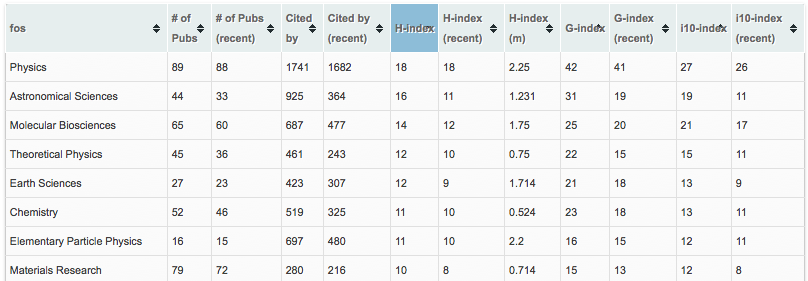
\includegraphics[width=1.0\columnwidth]{images/XDPUBS_Metrics_FOS.png}
  \caption{Metrics in FOS level}\label{F:xdpubs-metrics-fos}
\end{figure}

By using the user submitted publication entries only, which are tagged as `direct' output of XSEDE projects, we were able to show the `direct' impact of XSEDE. E.g., as of Jan 27, 2014, the 837 publications involved 882 XSEDE users as authors, and 220 organizations, 331 XSEDE projects, and received 11,258 citations to date. We have calculated the various metrics on the level of user, organization, projects, and FOS involved. Figure \ref{F:xdpubs-metrics-fos} shows the top most impact FOSes judging by h-index values.

\subsection{Project metrics vs SUs allocation}

\begin{figure}[htb]
  \centering
    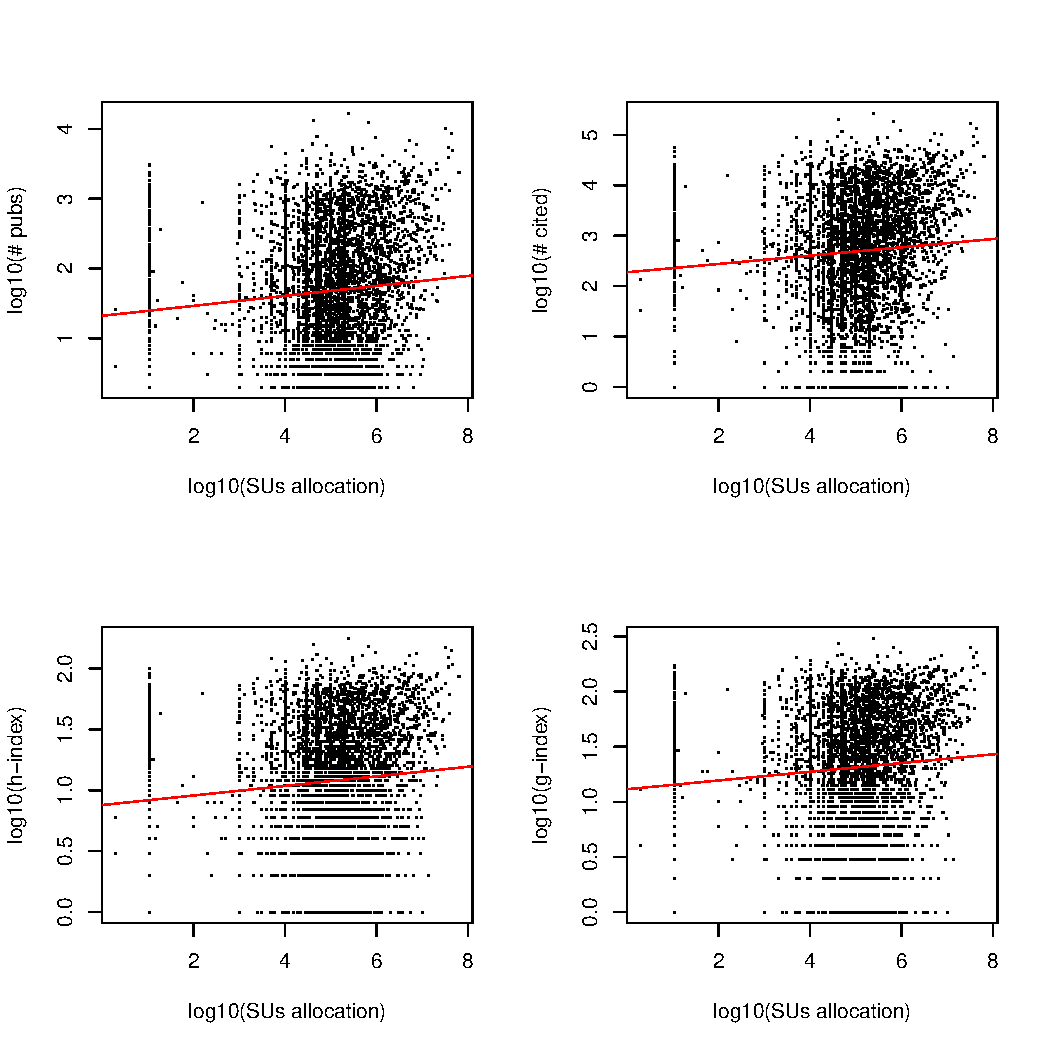
\includegraphics[width=1.0\columnwidth]{images/02_metrics_vs_alloc_proj.pdf}
  \caption{Metrics vs SUs for all projects}\label{F:metrics-vs-alloc-proj}
\end{figure}

\begin{figure}[htb]
  \centering
    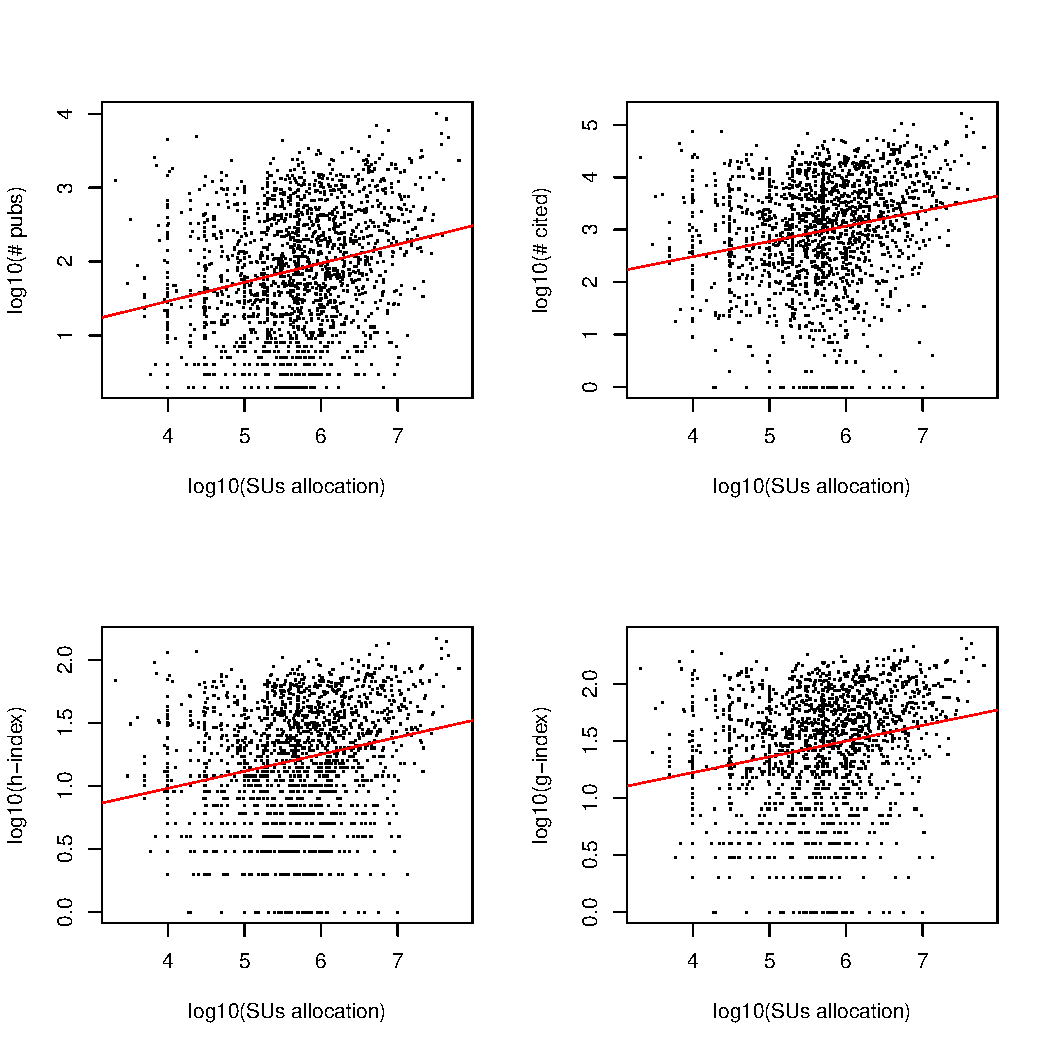
\includegraphics[width=1.0\columnwidth]{images/02_metrics_vs_alloc_research_proj.pdf}
  \caption{Metrics vs SUs for research projects}\label{F:metrics-vs-alloc-research-proj}
\end{figure}

%\begin{figure}[htb]
%  \centering
%    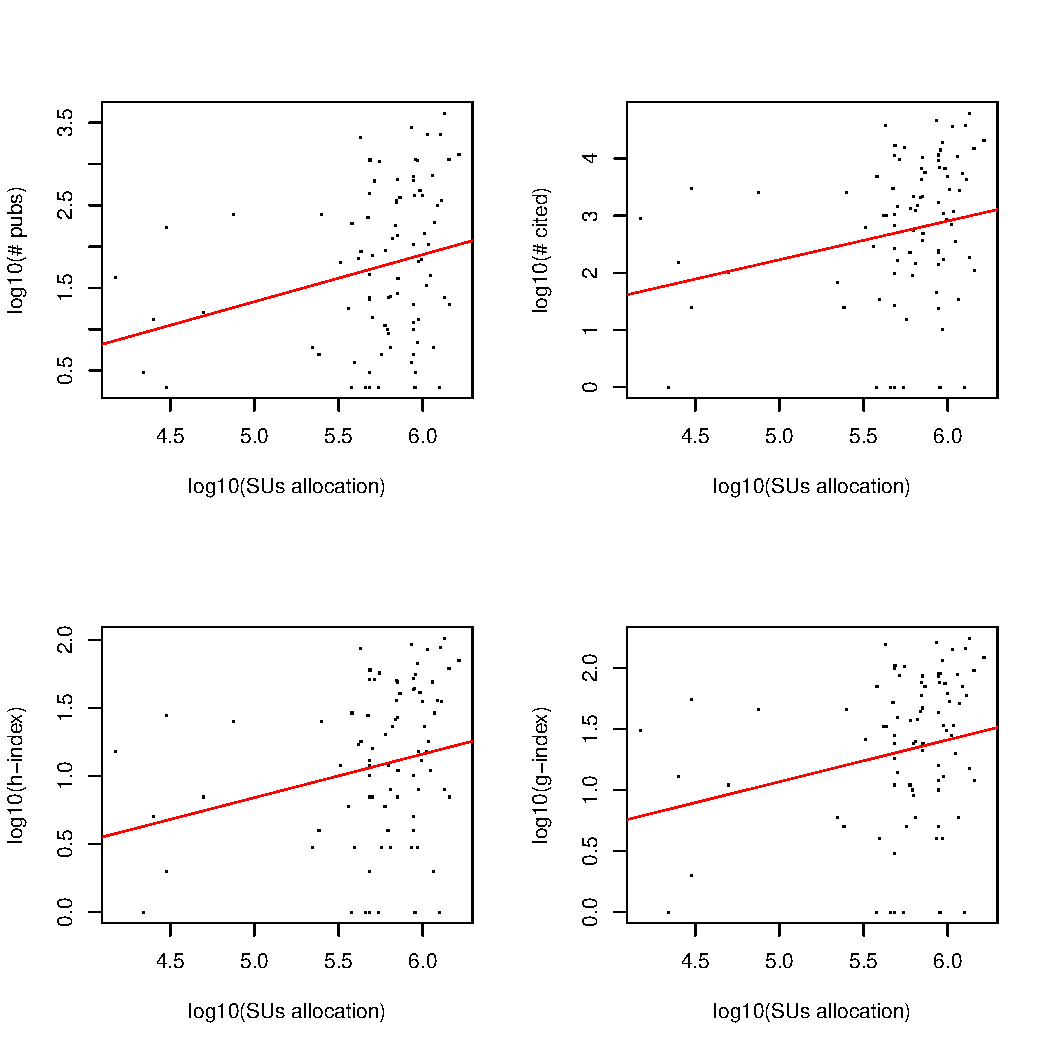
\includegraphics[width=1.0\columnwidth]{images/02_metrics_vs_alloc_campus_proj.pdf}
%  \caption{Metrics vs SUs for campus champion projects}\label{F:metrics-vs-alloc-campus-proj}
%\end{figure}

%\begin{figure}[htb]
%  \centering
%    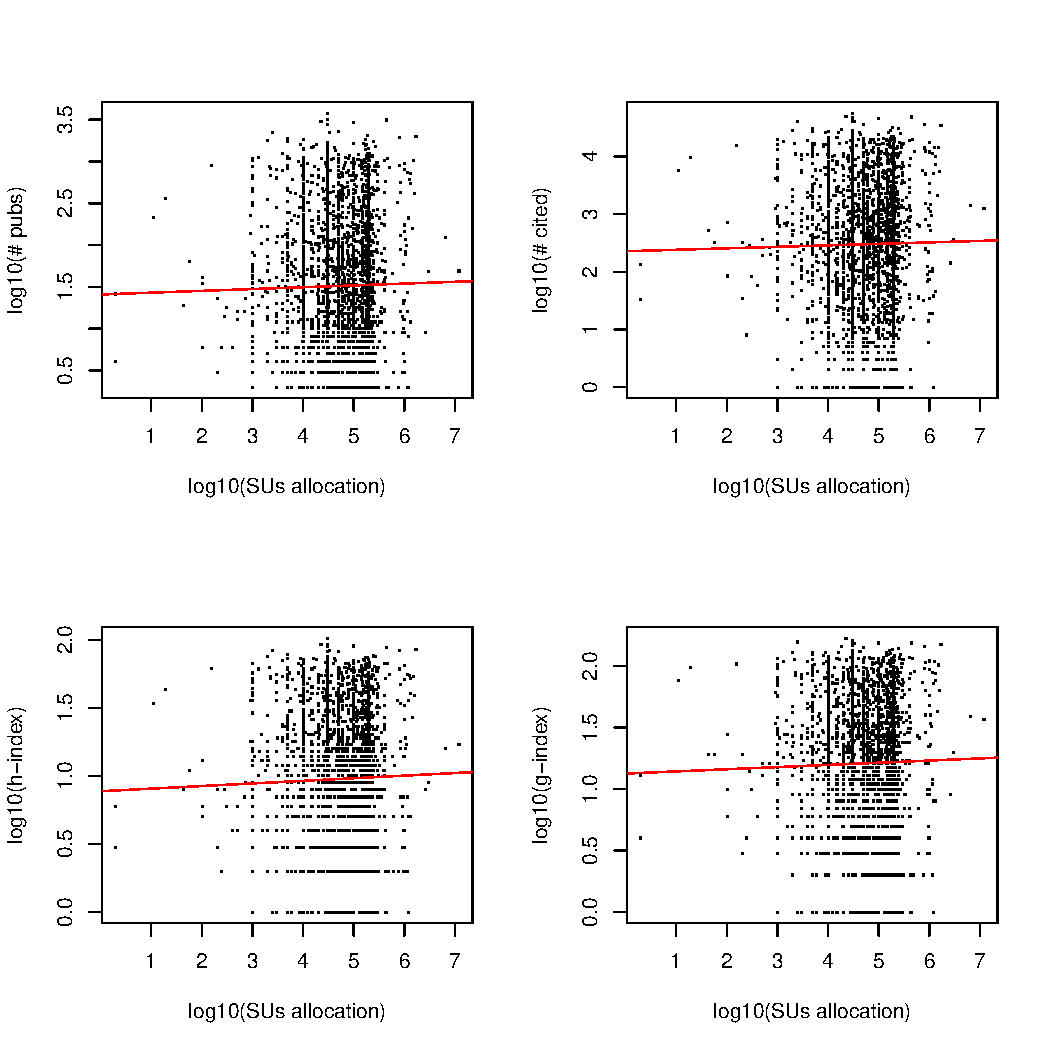
\includegraphics[width=1.0\columnwidth]{images/02_metrics_vs_alloc_startup_proj.pdf}
%  \caption{Metrics vs SUs for startup projects}\label{F:metrics-vs-alloc-startup-proj}
%\end{figure}

\begin{table}[htb]
  \centering
    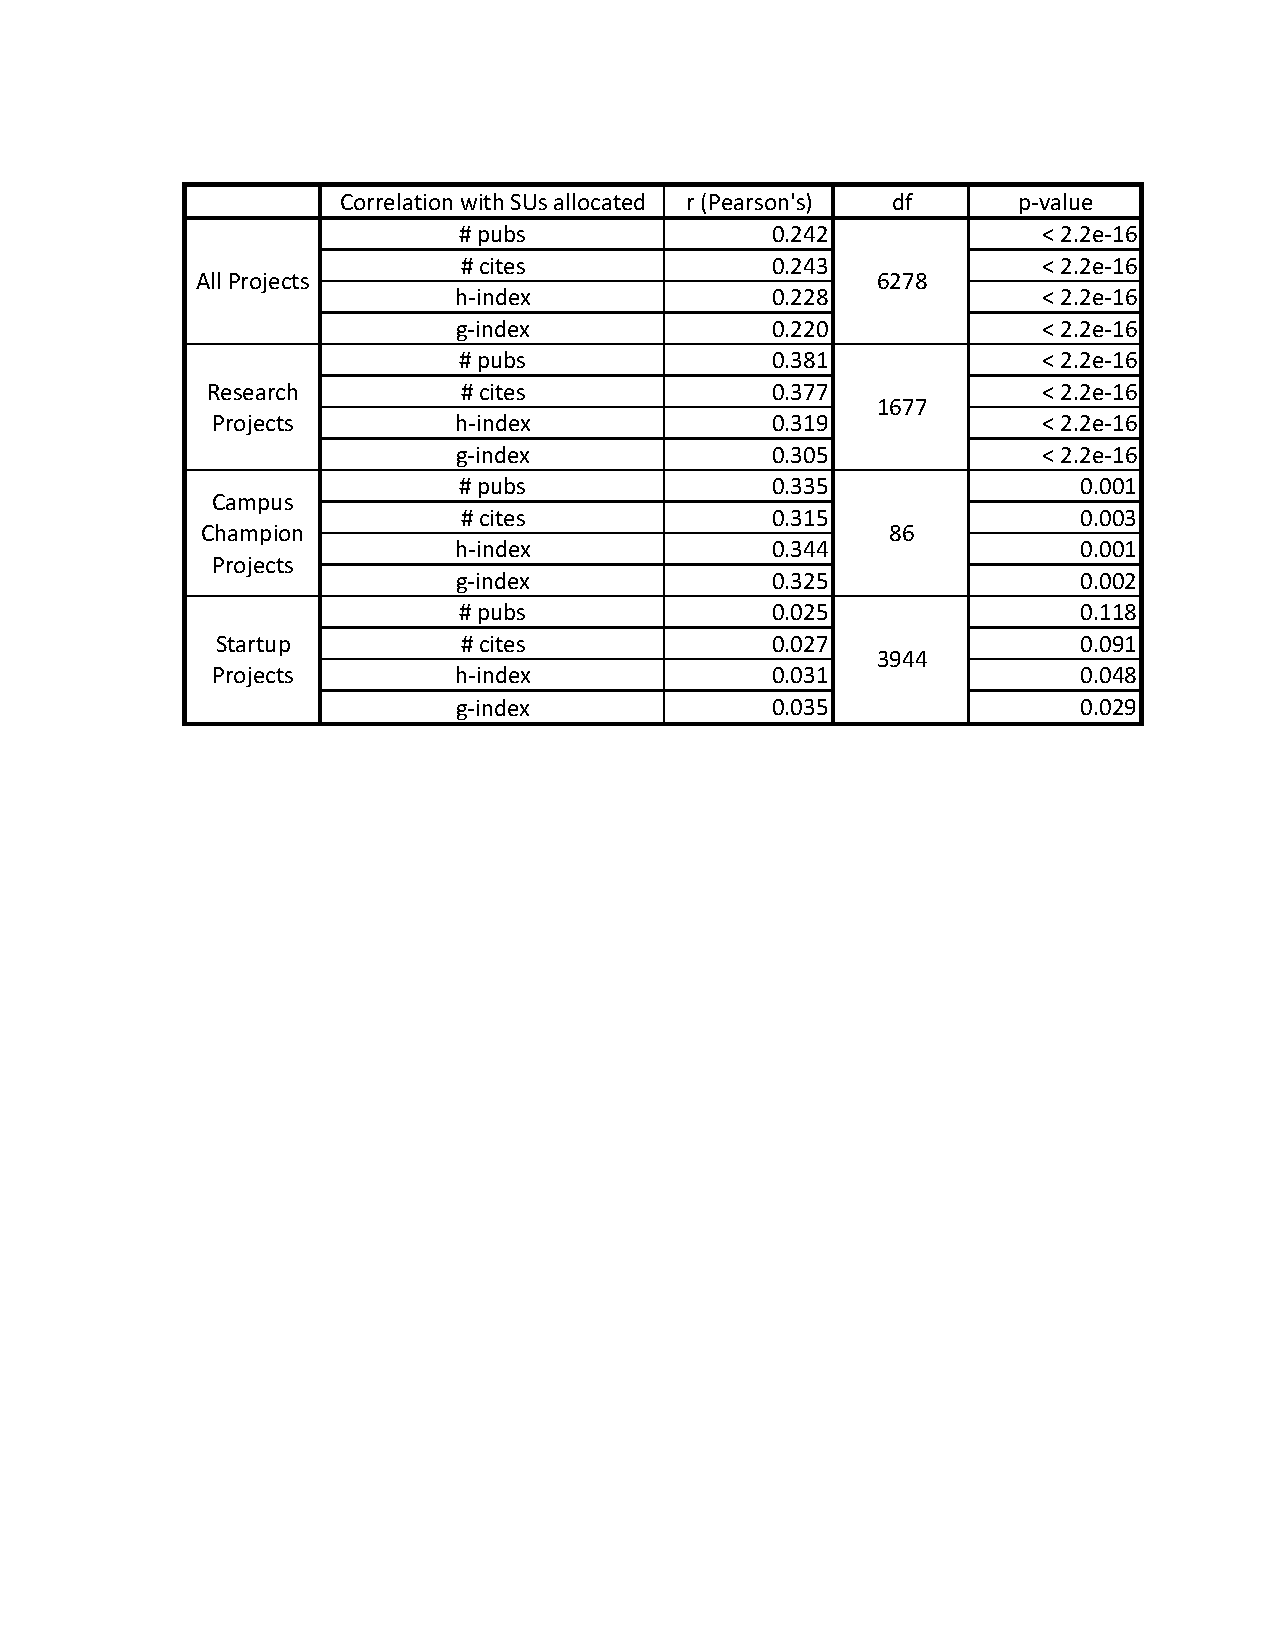
\includegraphics[width=1.0\columnwidth]{images/metrics_alloc_r.pdf}
  \caption{Correlation between SUs allocated vs the metrics for each project}\label{F:metrics-alloc-r}
\end{table}

Figure \ref{F:metrics-vs-alloc-proj} showed the correlation analysis of impact metrics and XD resource allocation on individual project level based on all projects data. While previous work showed stronger correlation between the citation and SUs \cite{bollen2011and} in much smaller sample size from one certain resource allocation meeting, we observed weaker correlation, if any. When categorizing the projects based on the types, e.g., research, startup, campus champion, etc., it shows a stronger, although still not strong, correlation in each category other than for the startup projects. Figure \ref{F:metrics-vs-alloc-research-proj} showed the analysis for research projects only. Table \ref{F:metrics-alloc-r} listed the correlation coefficient values as well as the p-values showing the significance of the test. Please note in Figure \ref{F:metrics-vs-alloc-proj} and \ref{F:metrics-vs-alloc-research-proj} we included a regression lines showing the upper trends of the correlation, i.e., higher SUs allocation correlating to higher impact metrics, but not suggesting the linear relationship. This correlation analysis does not show the cause effect either, as in this case it's very likely that the causal are reciprocal.

\subsection{Metrics vs SUs allocation on FOS level}

\begin{figure}[htb]
  \centering
    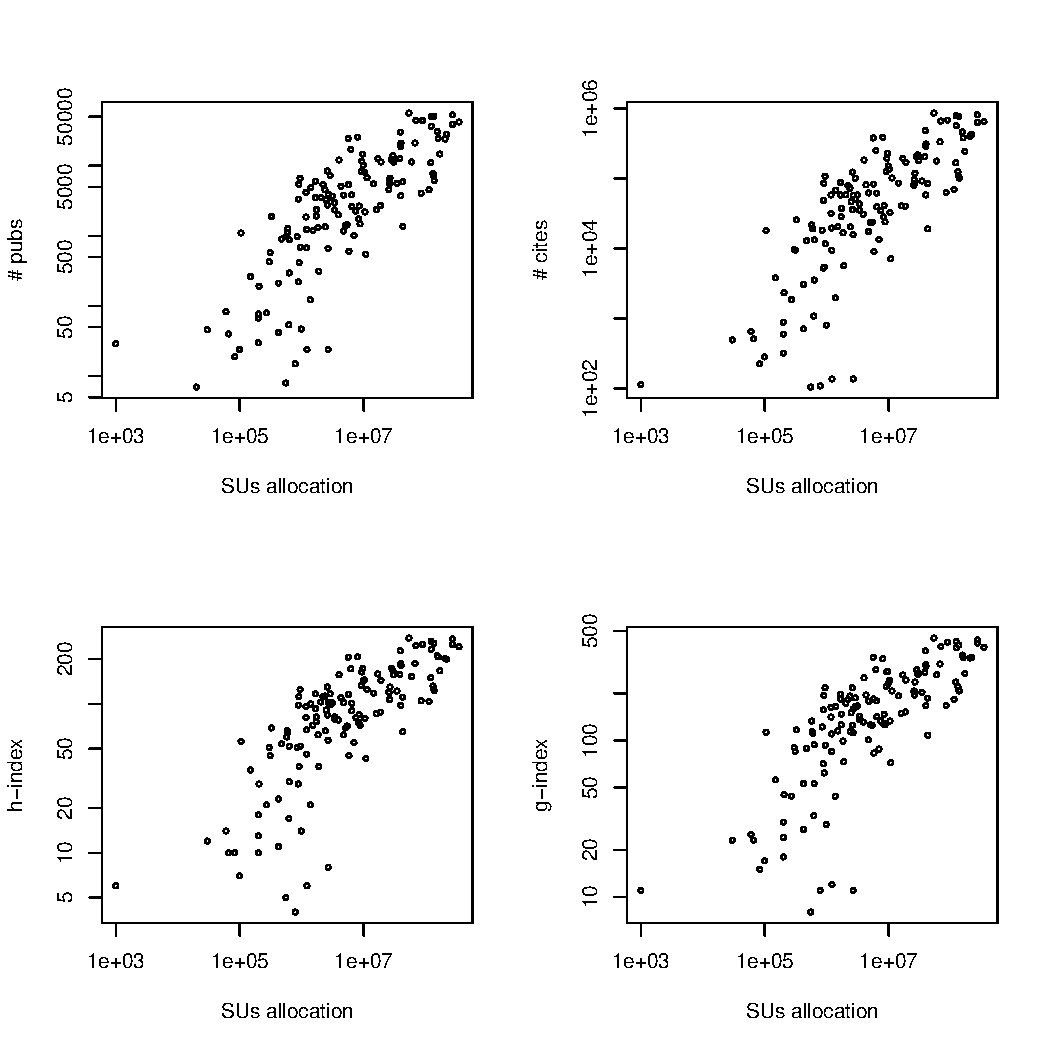
\includegraphics[width=1.0\columnwidth]{images/03_metrics_vs_alloc_fos.pdf}
  \caption{Metrics vs SUs for FOSes}\label{F:metrics-vs-alloc-fos}
\end{figure}
While on individual project level we don't observe strong correlations between impact metrics vs the resource allocations, Figure \ref {F:metrics-vs-alloc-fos} shows stronger positive correlation on FOS level. The Pearson correlation coefficient are 0.704, 0.712, 0.651, 0.648 respectively. With a degree of freedom at 132 and p-values less than 2.2e-16 from the test, it shows very high statistical significance. 

%\begin{figure}[htb]
%  \centering
%    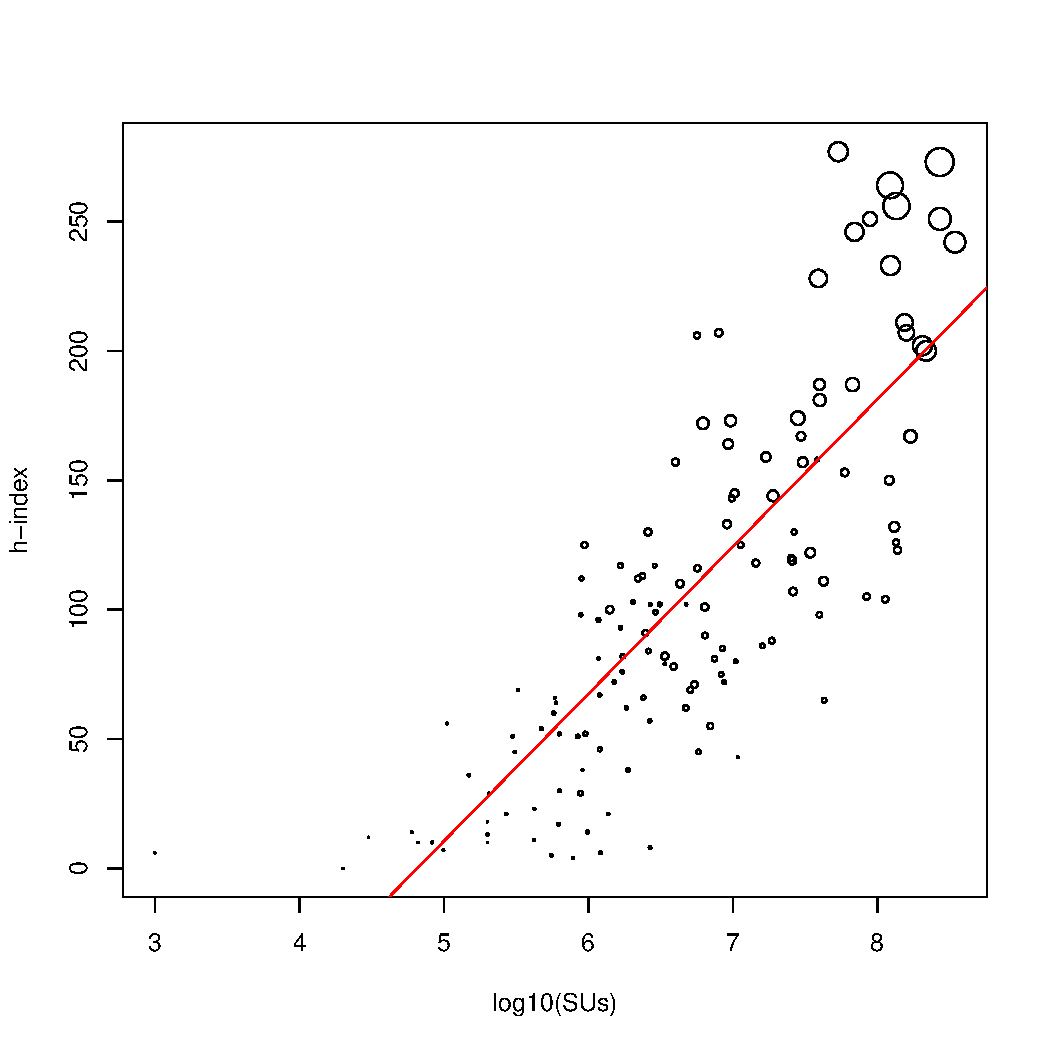
\includegraphics[width=1.0\columnwidth]{images/04_hindex_vs_alloc_fos_sized.pdf}
%  \caption{h-index (sized by size of FOS) vs allocation}\label{F:hindex-vs-alloc-fos-sized}
%\end{figure}

\begin{figure}[htb]
  \centering
    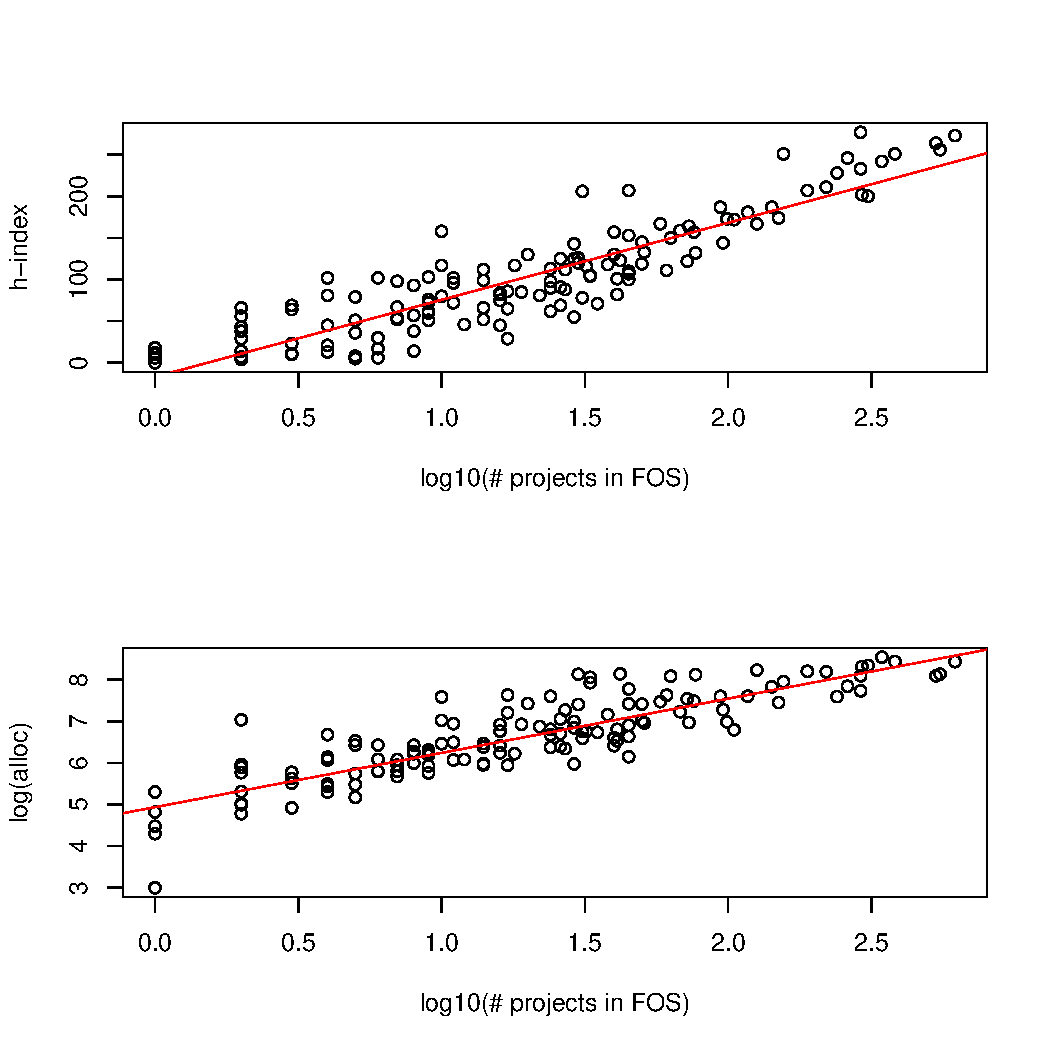
\includegraphics[width=1.0\columnwidth]{images/05_hindexalloc_vs_nprojects_fos_trended.pdf}
  \caption{Effects of sizes of FOSes}\label{F:hindexalloc-vs-nprojects-fos-trended}
\end{figure}

However as Figure \ref{F:hindexalloc-vs-nprojects-fos-trended} suggests, the stronger correlations are mostly caused by the effect of different size of the FOSes, judging by number of projects each FOS has. But this does not diminish the purpose of the analysis showing how XSEDE could impact science from different disciplines, e.g., by approving more projects and granting more allocations for certain FOSes.

\begin{figure}[htb]
  \centering
    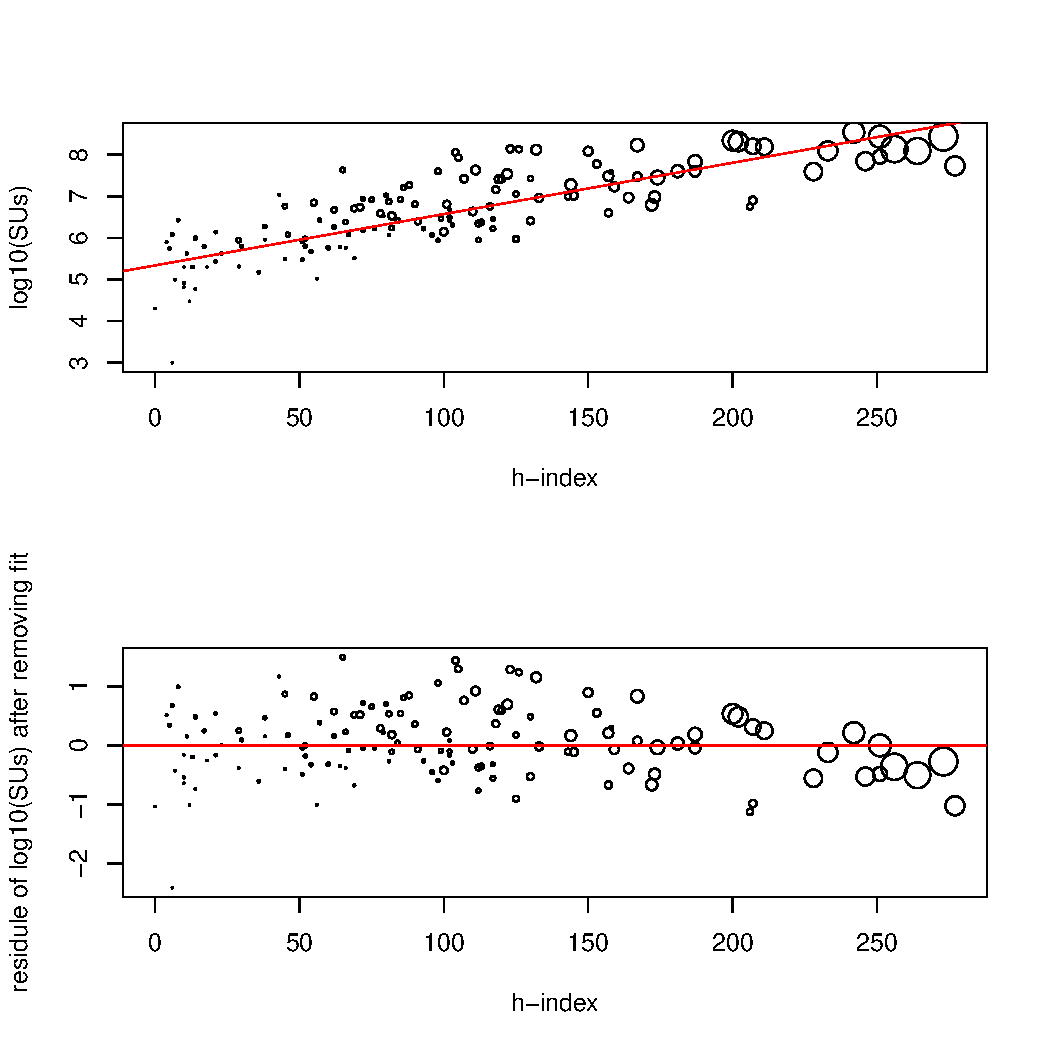
\includegraphics[width=1.0\columnwidth]{images/05_alloc_vs_hindex_fos_sized_2in1.pdf}
  \caption{SUs vs h-index for each FOS with trend (above) and residual analysis (bottom)}\label{F:alloc-vs-hindex-fos-sized}
\end{figure}

%\begin{figure}[htb]
%  \centering
%    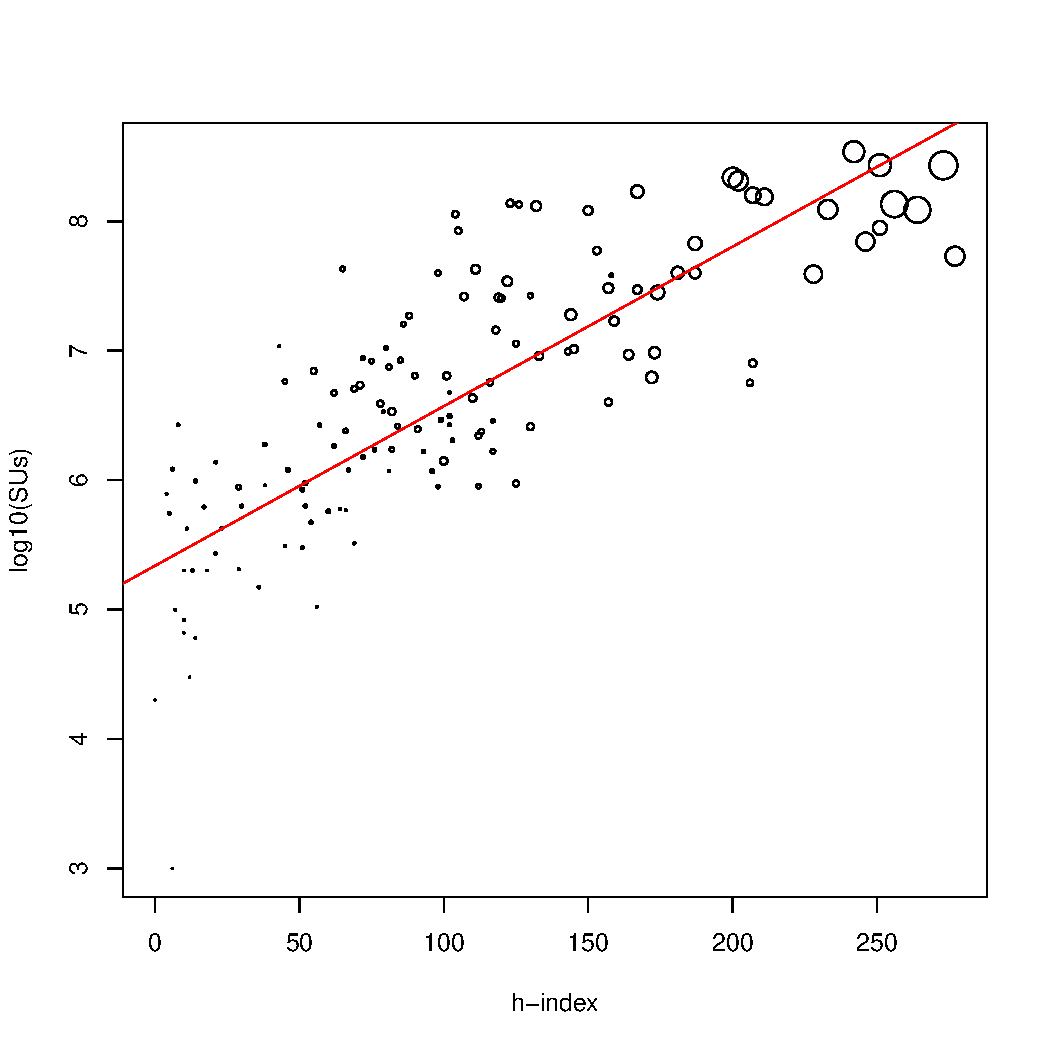
\includegraphics[width=1.0\columnwidth]{images/05_alloc_vs_hindex_fos_sized_trended.pdf}
%  \caption{SUs vs h-index for each FOS with trend}\label{F:alloc-vs-hindex-fos-sized-trended}
%\end{figure}

%\begin{figure}[htb]
%  \centering
%    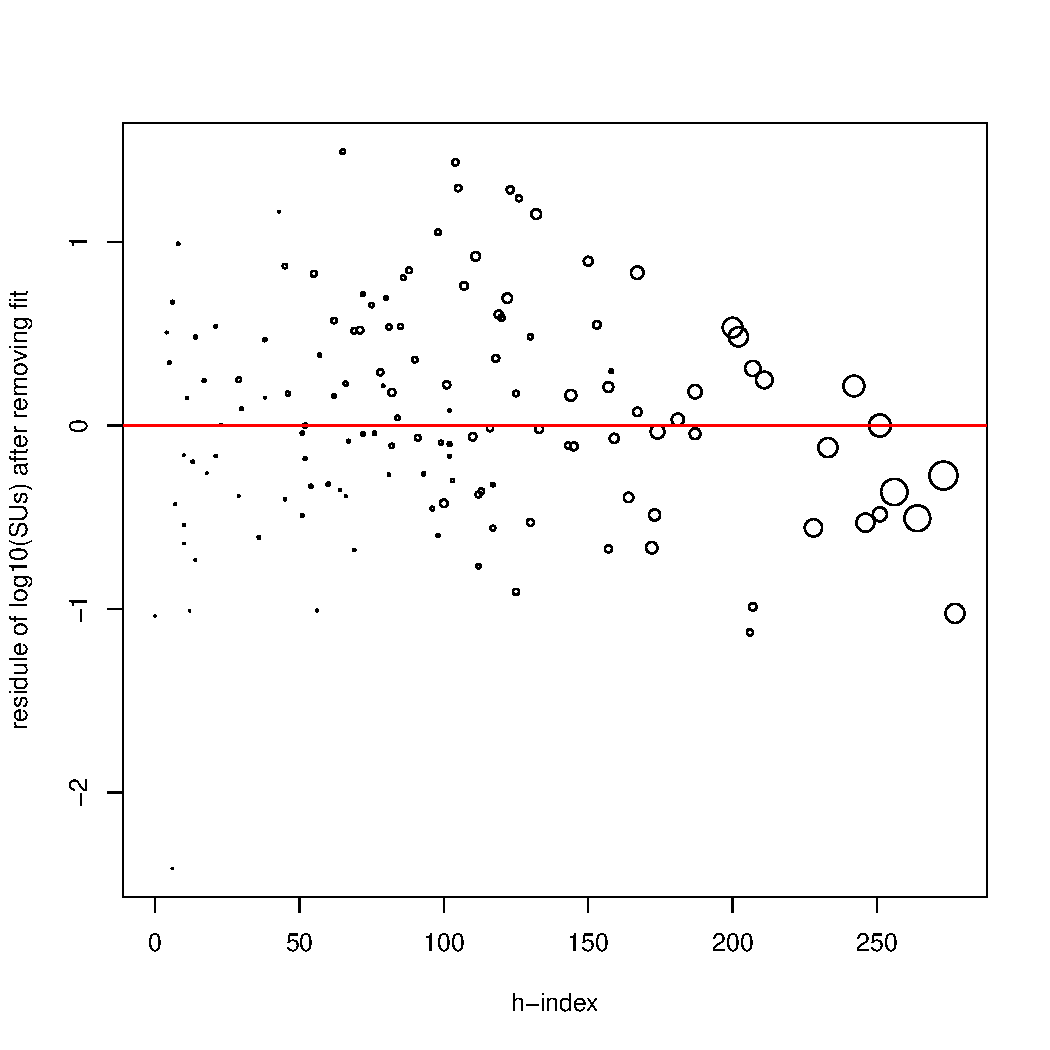
\includegraphics[width=1.0\columnwidth]{images/05_alloc_vs_hindex_fos_sized_residual.pdf}
%  \caption{Residual analysis of SUs vs h-index}\label{F:alloc-vs-hindex-fos-sized-residual}
%\end{figure}

\begin{figure}[htb]
  \centering
    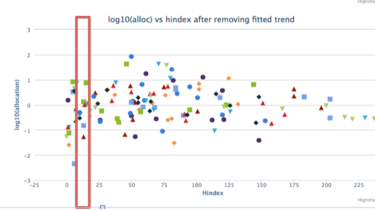
\includegraphics[width=1.0\columnwidth]{images/fig3.pdf}
  \caption{Interactive SUs vs h-index on FOS level}\label{F:fig3}
\end{figure}

Figure \ref{F:alloc-vs-hindex-fos-sized} showed the SUs received (transformed in logarithmic scale) vs the h-index produced for each FOS, while the circle size proportional to the size (number of projects) of the FOS. It also showed that after removing the fitted trend, we could see the diverging of the SUs received, from the expected SUs trend to produce the given impact judging by h-index. This could imply that certain FOSes are more efficiently to produce the given impact while some others are requiring more than expected SUs to produce the given impact. To further facilitate this analysis, we have an interactive version of the plot in our web portal as shown in Figure \ref{F:fig3}. It helps to make the following observations:

\begin{enumerate}

\item We find that several FOS with the similar h-index use fewer resources than others showing better relative output measured by the h-index. This is done by comparing FOS on a vertical slice of the h-index as seen in Figure \ref{F:fig3}

\item The trend introduces a baseline of 0. FOS above 0 use more resources than the trend, FOS bellow 0 use less resources to produce the expected impact based on a given h-index.

\item Some outliers might need more careful investigation, e.g., if more supports should be given to projects in that FOS?

\end{enumerate}

\begin{figure}[htb]
  \centering
    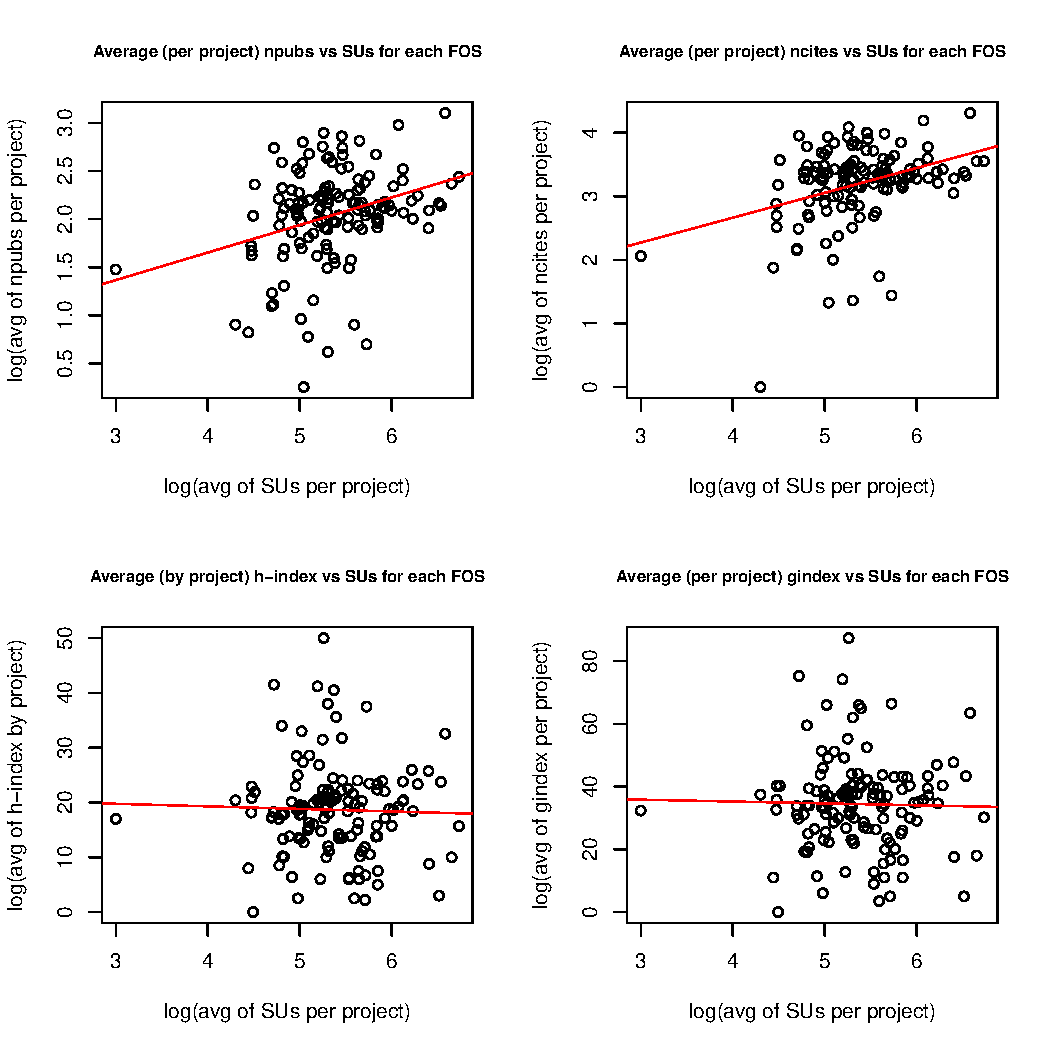
\includegraphics[width=1.0\columnwidth]{images/08_metrics_vs_alloc_avg_log_fit.pdf}
  \caption{Metrics vs SUs for FOS (avg by project)}\label{F:metrics-vs-alloc-avg-log-fit}
\end{figure}

\begin{table}[htb]
  \centering
    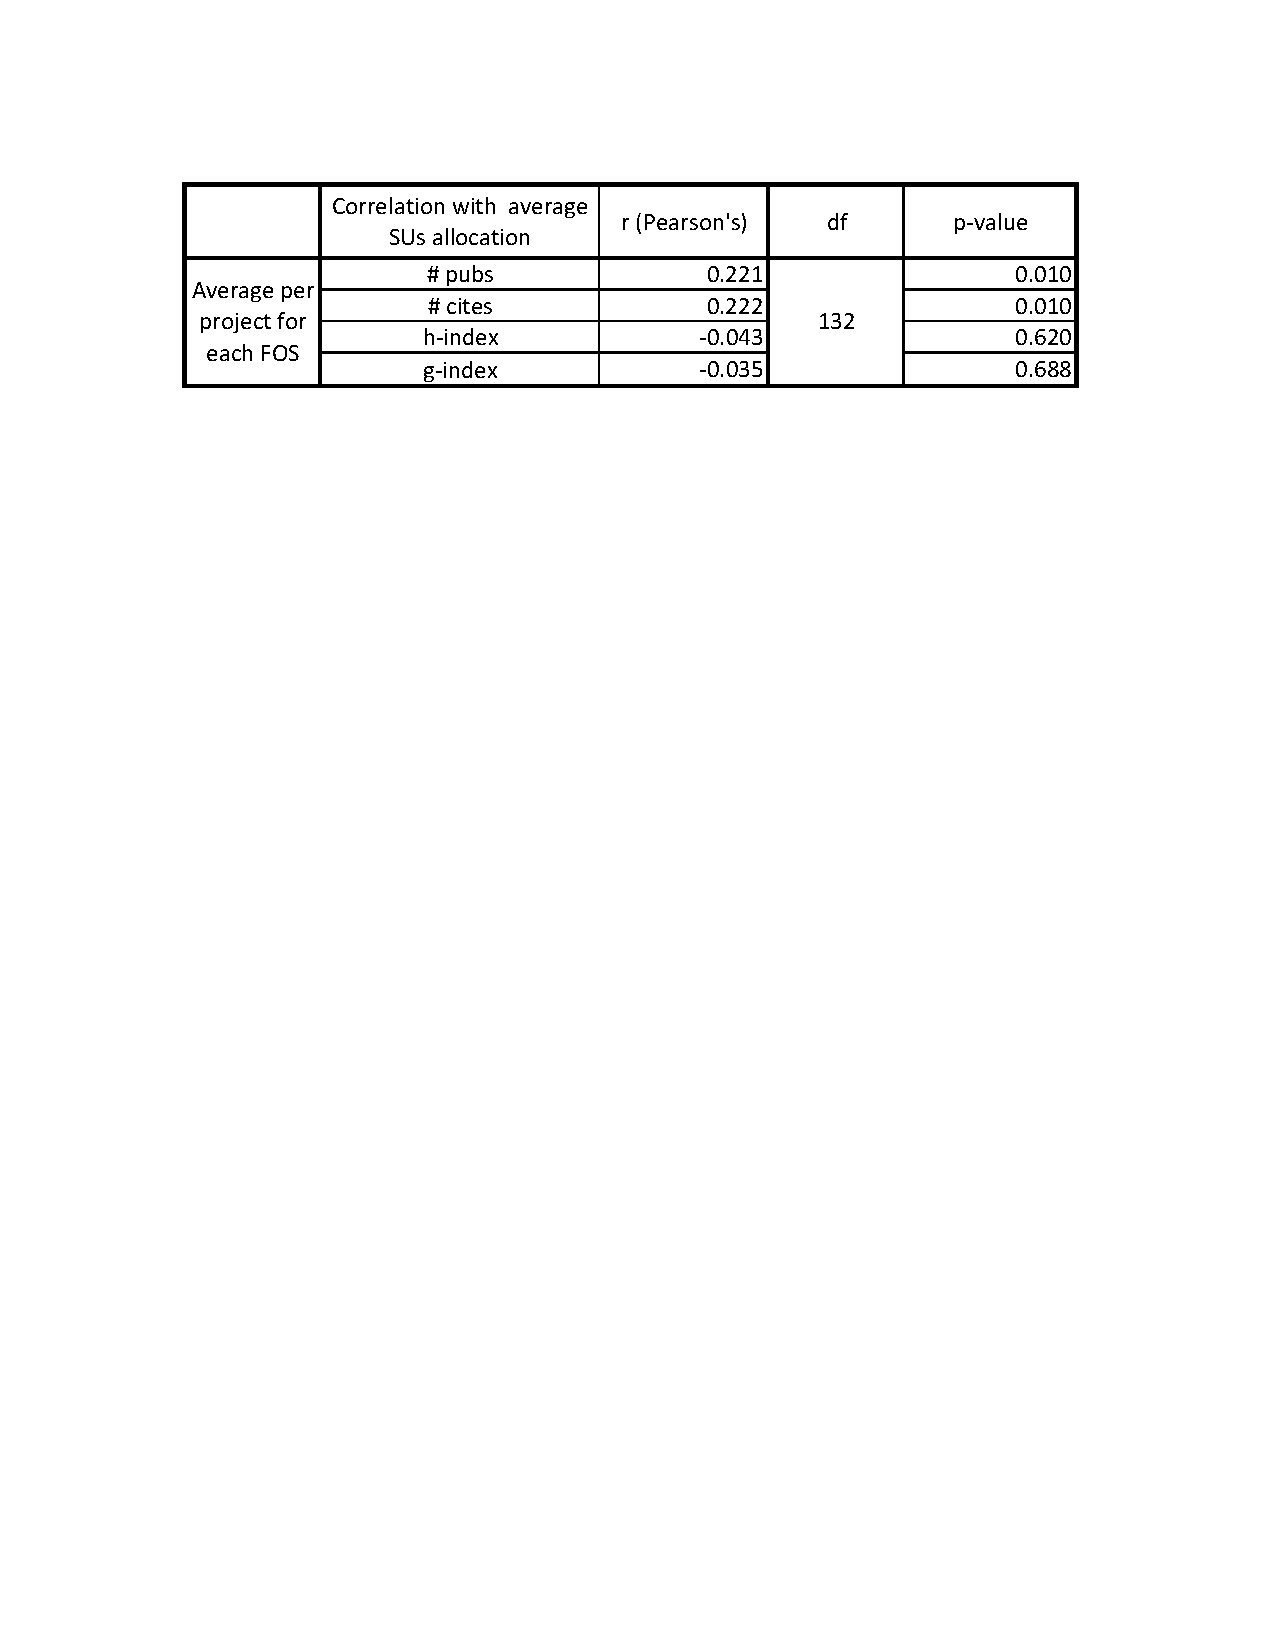
\includegraphics[width=1.0\columnwidth]{images/metrics_alloc_r_fos.pdf}
  \caption{Correlation between average SUs allocated vs the average metrics (by projects) for each FOS}\label{F:metrics-alloc-r-fos}
\end{table}

As size of FOS affects significantly the impact as well as the allocations, e.g. for h-index as in Figure \ref{F:hindexalloc-vs-nprojects-fos-trended}. We can eliminate this effect by comparing the averaging by project values within each FOS, as shown in Figure \ref{F:metrics-vs-alloc-avg-log-fit}. Table \ref{F:metrics-alloc-r-fos} has the values. It shows the weak correlation of per project based metrics vs SUs for number of publications and citations, which is actually not significantly different than the result from Table \ref{F:metrics-alloc-r}. For h-index and g-index, the test implies no correlation at all found probably due to the case that these metrics does not work well when averaging as they are not cumulative and additive values.

\begin{figure}[htb]
  \centering
    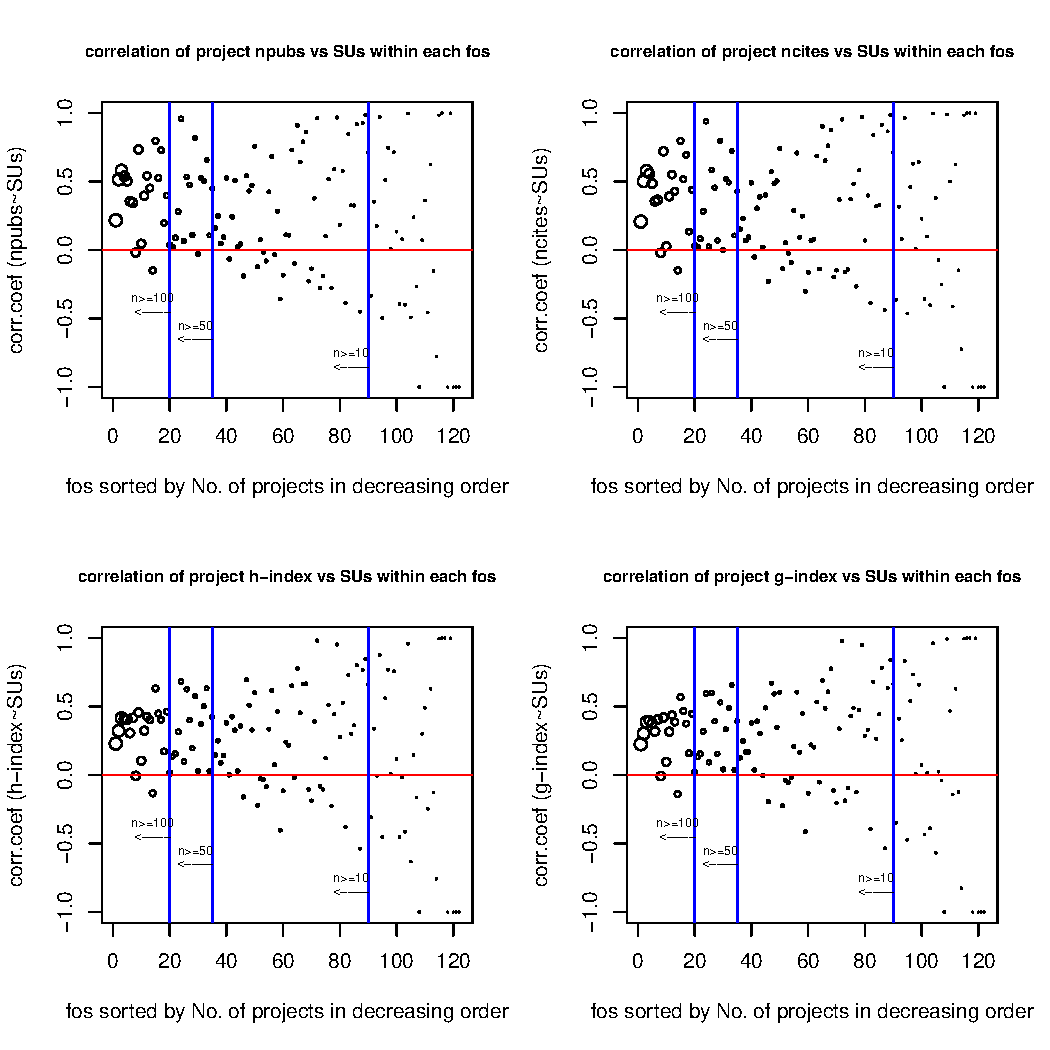
\includegraphics[width=1.0\columnwidth]{images/06_corr_metrics_vs_alloc_proj_by_fos.pdf}
  \caption{Correlations of metrics vs SUs on project level for each FOS}\label{F:corr-metrics-vs-alloc-proj-by-fos}
\end{figure}

However as shown in Figure \ref{F:corr-metrics-vs-alloc-proj-by-fos}, within each FOS, the project level metrics vs SUs correlations are typically a bit higher especially for those large size FOSes. With the increasing of size of FOS (n=10, n=50, and n=100) are denoted as vertical lines), the correlation appears positively higher and more significant. This suggests that for most FOS, impact metrics does have positive correlations with SUs allocated. Also by investigating the individual data points, we could see in which FOS this correlation appears much stronger, while for some others there are not correlation at all.

%\begin{figure}[htb]
%  \centering
%    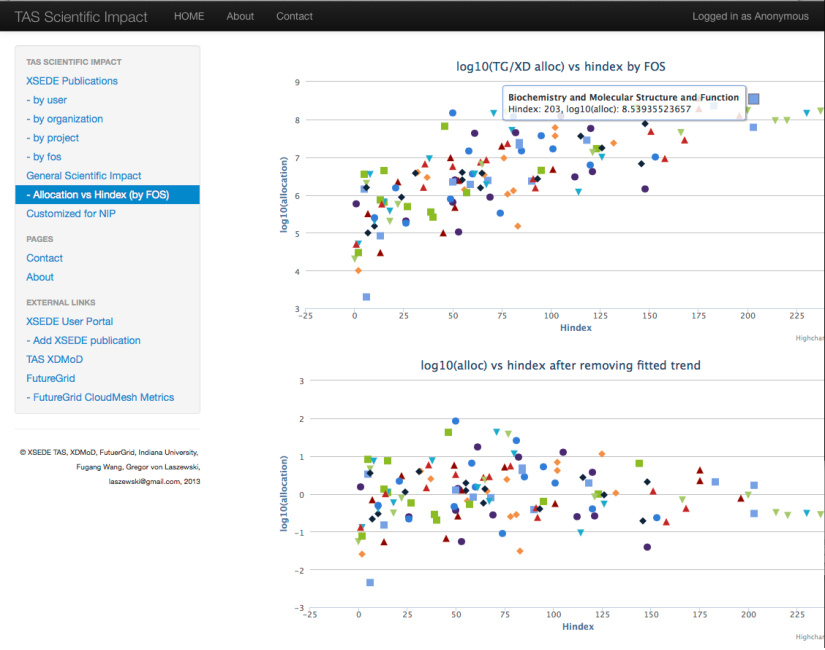
\includegraphics[width=1.0\columnwidth]{images/fig2.pdf}
%  \caption{fig2.}\label{F:fig2}
%\end{figure}

%\begin{figure}[htb]
%  \centering
%    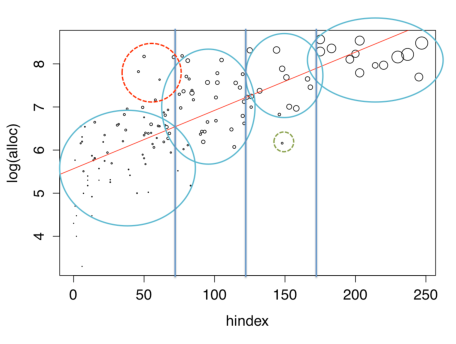
\includegraphics[width=1.0\columnwidth]{images/fig4.pdf}
%  \caption{fig4.}\label{F:fig4}
%\end{figure}

%\begin{figure*}[htb]
%  \centering
%    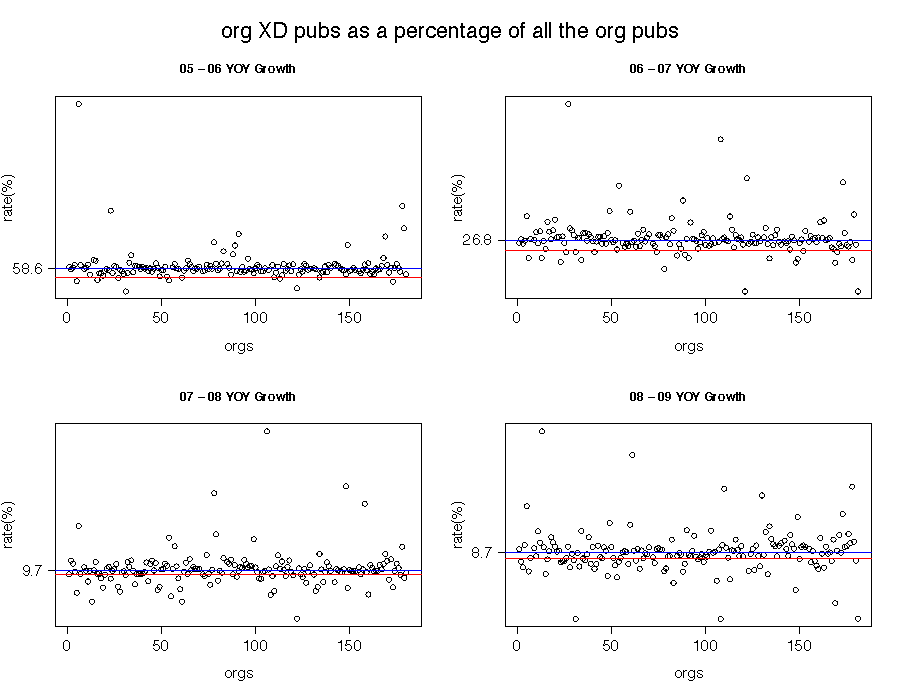
\includegraphics[width=1.0\textwidth]{images/fig5.pdf}
%  \caption{fig5.}\label{F:fig5}
%\end{figure*}

% from previous summary report

%\begin{figure}[htb]
%  \centering
%    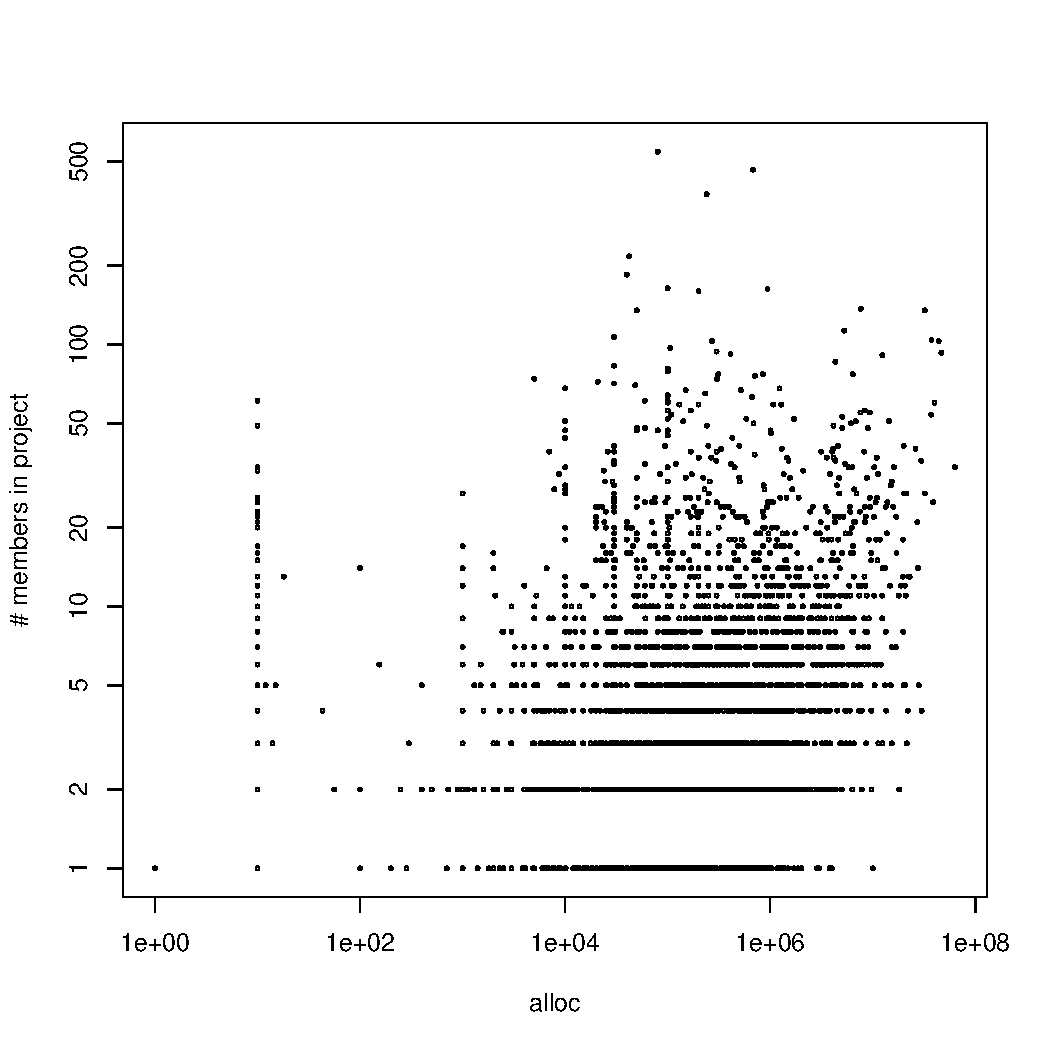
\includegraphics[width=1.0\columnwidth]{images/02_nmembers_vs_alloc_proj.pdf}
%  \caption{fig3.}\label{F:nmembers-vs-alloc-proj}
%\end{figure}

%\begin{figure}[htb]
%  \centering
%    \includegraphics[width=1.0\columnwidth]{images/05_alloc_vs_nprojects_fos_trended.pdf}
%  \caption{fig3.}\label{F:alloc-vs-nprojects-fos-trended}
%\end{figure}

%\begin{figure}[htb]
%  \centering
%    \includegraphics[width=1.0\columnwidth]{images/05_hindex_vs_nprojects_fos_trended.pdf}
%  \caption{fig3.}\label{F:hindex-vs-nprojects-fos-trended}
%\end{figure}

%\begin{figure}[htb]
%  \centering
%    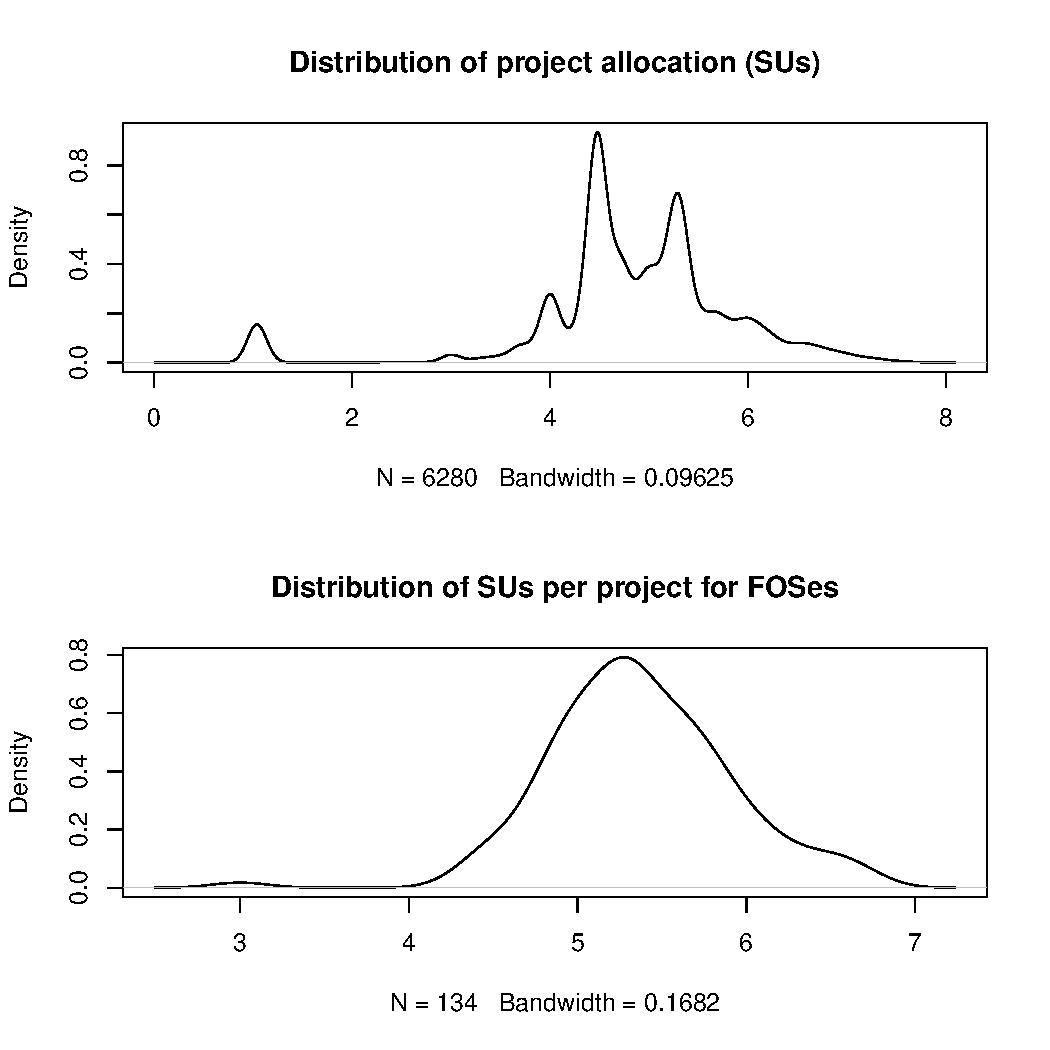
\includegraphics[width=1.0\columnwidth]{images/07_density_alloc.pdf}
%  \caption{fig3.}\label{F:density-alloc}
%\end{figure}

%\begin{figure}[htb]
%  \centering
%    \includegraphics[width=1.0\columnwidth]{images/07_density_alloc_fos_avg_by_nprojs.pdf}
%  \caption{fig3.}\label{F:density-alloc-fos-avg-by-nprojs}
%\end{figure}

%\begin{figure}[htb]
%  \centering
%    \includegraphics[width=1.0\columnwidth]{images/07_density_alloc_proj.pdf}
%  \caption{fig3.}\label{F:density-alloc-proj}
%\end{figure}
